% Page: Functions of random variables and limit theorems
% sources/stat2003/chapters/prob-05-transforms-and-limits.qmd
% Exact density of the standardised sum (S_n - n mu)/(sigma sqrt(n))
% when the summands are Exp(1), so mu = sigma = 1. The sum of n such
% variables is Gamma(n, rate 1). The dashed curve is the N(0,1) density,
% whose distribution function is the Phi in the central limit theorem.
\documentclass[border=6pt]{standalone}
\usepackage[T1]{fontenc}
\usepackage{lmodern}
\usepackage{amsmath,amssymb}
\usepackage{tikz}
\usepackage{pgfplots}
\pgfplotsset{compat=1.18}
\definecolor{ink}{HTML}{1F2430}
\definecolor{statblue}{HTML}{174A7E}
\definecolor{grey}{HTML}{5E6A75}
\pgfplotsset{
  stat/.style={
    scale only axis,
    axis lines=left,
    axis line style={ink, line width=0.6pt},
    tick style={ink, line width=0.45pt},
    tick label style={font=\small, text=ink},
    label style={font=\small, text=ink},
    title style={font=\small, text=ink, align=center},
    legend style={font=\small, draw=none, fill=none, text=ink,
      cells={anchor=west}, inner sep=1.5pt,
      at={(0.98,0.98)}, anchor=north east},
    unbounded coords=jump,
    scaled ticks=false,
    every axis plot/.append style={line width=0.9pt, line join=round},
  },
}
\begin{document}
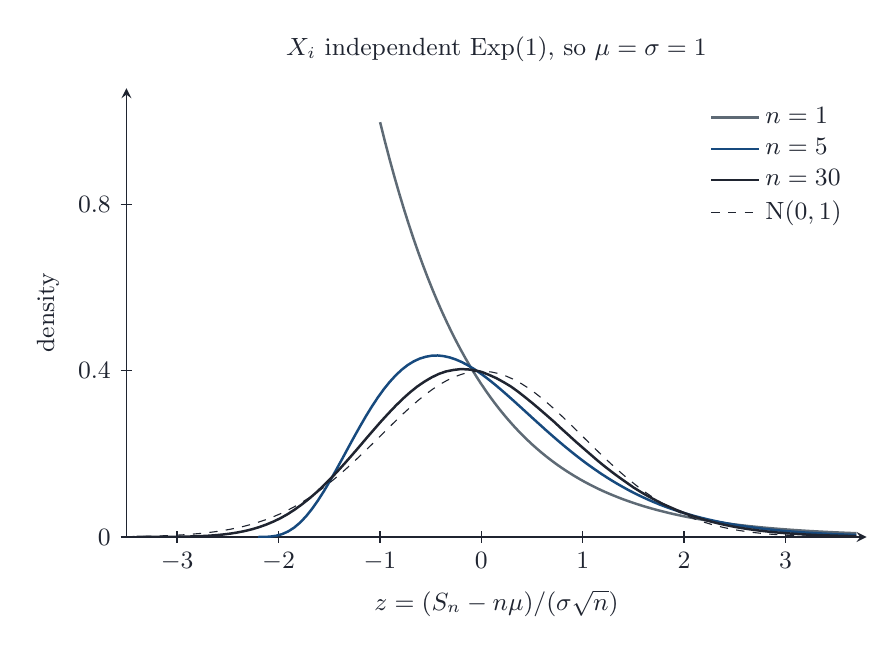
\begin{tikzpicture}
\begin{axis}[
  stat, width=9.4cm, height=5.7cm,
  xmin=-3.5, xmax=3.8, ymin=0, ymax=1.08,
  xtick={-3,-2,-1,0,1,2,3},
  ytick={0,0.4,0.8},
  xlabel={$z=(S_n-n\mu)/(\sigma\sqrt{n})$},
  ylabel={density},
  title={$X_i$ independent $\operatorname{Exp}(1)$, so $\mu=\sigma=1$},
  samples=101,
]
  \addplot[grey, domain=-0.998:3.7] {exp(-(x+1))};
  \addlegendentry{$n=1$}
  % log-density of Gamma(n, rate 1), standardised. ln((n-1)!) = lgamma(n).
  \addplot[statblue, domain=-2.2:3.7] {%
    exp(4*ln(5+x*sqrt(5))-(5+x*sqrt(5))-3.1780538303+0.5*ln(5))};
  \addlegendentry{$n=5$}
  \addplot[ink, domain=-3.4:3.7] {%
    exp(29*ln(30+x*sqrt(30))-(30+x*sqrt(30))-71.2570389672+0.5*ln(30))};
  \addlegendentry{$n=30$}
  \addplot[ink, dashed, thin, domain=-3.5:3.7] {exp(-x^2/2)/sqrt(2*pi)};
  \addlegendentry{$\operatorname{N}(0,1)$}
\end{axis}
\end{tikzpicture}
\end{document}
